\documentclass[12pt]{article}
\title{A Survey of Error Correcting Codes in Computer Networks}
\author{Daniel Kearney}
\date{October 30, 2018}
\usepackage[margin=1in,footskip=0.25in]{geometry}
\usepackage[pdftex]{graphicx}
\usepackage{amsmath}
\usepackage{float}
\usepackage{longtable}


\begin{document}

\maketitle

\section{Introduction}

Communication is inherently noisy. From a noisy restaurant to an underwater fiber, the real world does not always cooperate with our attempts to send data. Error correction is a fascinating suite of technologies that allows us to send data through noisy channels and actually recover data that was changed by noise, at the cost of reduced bandwidth. These technologies are particularly critical when sending data over noisy channels like WiFi and physical media like DVDs that can get dirty. In this paper, I present an overview of error correction codes, and discuss a few technologies in detail.

\section{Motivation for Error Correcting}

Error correcting codes are often discussed in tandem with error detection as they are similar. With error detection, a computation (like a checksum) is computed and attached to the data, and the receiver is tasked to compute the same computation; if the result of the computation does not match, then an error must have occurred. At that point, typically, the data would be re-transmitted. Why, then, do we have error correction?

There are several key scenarios where retransmission is not suitable. For example, networks with a high delay, like a satellite channel or a deep space probe, may have long times in transit and any retransmissions may significantly slow down the overall data rate. (Huffman 1) And for particularly noisy channels, like wireless networks, errors may be so common that retransmissions may become extremely common, again, eating into bandwidth as data is endlessly retransmitted. In the worst case, it could become very challenging to send data at all when errors become very common!

Perhaps the most important scenarios for error correction in static media. For example, on a DVD, there is no concept of a retransmission -- if a scratch causes bit errors, those errors are permanent. Server memory, likewise, has no guarantee of being able to be re-computed. In those use cases, error correction is nearly required to prevent data decay over time. \cite{pless}

Interestingly, there is rudimentary error correction built into the building blocks of life itself! Biological genomes are transcribed into proteins via RNA-amino acid coding. These codes turn triplets of amino acids -- like AUG, CCU, GAG -- into proteins. There are 4 basic amino acids, and so there are 64 possible triplets. However, there are only 20 amino acids. Many amino acids can be transcribed with multiple different triplets. This means that an error in DNA or RNA -- if it does not change the output protein -- can be recovered from harmlessly. While this is not true error correction, this resiliency to error is fascinating. \cite{wolf}

\section{Background}

Error Control Codes were first laid out by Claude Shannon, the founder of information theory, who posited that data transmitted through a noisy channel, with a suitable encoding, could be guaranteed to have a certain accuracy -- with the cost that additional bits of data may be used. Shannon, in that proof, did not lay out a specific algorithm or implementation, but rather the mathematical framework with which all practical error correcting codes. \cite{pless}

$\text{maximum number of bits/sec} = B\log 2 (1 + S/N)$ \cite{tanenbaum}

While this helps to understand the upper bounds of what's achievable with error correcting codes to achieve arbitrarily low bit error rates, Shannon left the actual implementations up to future work. This paper discusses some technologies in use today for error correcting.

\section{Background on Error Control}

\subsection{Types of Error Correction}

There are two main types of error correction codes used in practice. Block codes operate on fixed blocks of data length, while convolutional codes operate more like streams, producing a new set of output bits based on a sliding window lookback. 

Another distinction is hard versus soft decision codes. Hard decision codes definitively state an error occurred; soft decision codes utilize probabilities, saying that an error might have occurred with some probability. Soft decision codes are powerful because they provider richer information about errors. \cite{mitvit}

Convolutional Codes typically are more flexible for allowing soft decisions.\cite{tanenbaum}

\subsection{Terminology}

Input data is transformed via error correcting codes into codewords. A codeword is called systematic when the data bits themselves are present in the codewords; they are not systematical if the original data is not present. 

The Hamming distance is defined as the number of components that they are different. The Hamming distance is used to measure how many errors can be corrected or detected for a given code. For example, two codewords with a Hamming distance of one only differ by a single bit. In that case, the two codewords can be shown to have one bit error from each other. Likewise, a Hamming (7, 4) code has a Hamming distance of 3, making it possible to correct one error. An extended Hamming code has a distance of 4, making it possible to correct one error and definitely detect two others. \cite{sphere}

\section{Block Codes}

\subsection{Simple Error Control Using Redundant Data}

As a trivial example, imagine trying to send the binary sequence 010101 through a noisy channel that's prone to flipping bits. The simplest mechanism for error detection would be to send each bit twice; therefore if two bits that should agree do not, then one of them has flipped. This however does not help much with error correction, because we don't know which is correct! So the simplest mechanism is to send each bit three times: 000111000111000. This will guarantee that we can correct a single bit error and possibly several, but again, there are no guarantees beyond a single bit error. Obviously, this is a very poor code because we're using 3 bits to send 1 bit of data, which is a lot of overhead. In fact, the lower limit is defined as 

$(m + r + 1) ≤ 2 r (3-1)$ \cite{tanenbaum}

With our naive approach, we see that each bit requires a total of 3 bits to transmit 1 data bit, what we call a rate of 1/3. Hamming 4,7 codes achieve 4/7, Golay 12/23, and other get closer to 1/2. This limit is a consequence of the Shannon limit. \cite{pless}

\subsection{Hamming Codes (4, 7)}

Hamming codes are an improvement over pure redundancy that can correct single-bit errors using some clever math. 

A Hamming code utilizes a series of parity bits on segments of the data bits to verify the correctness of the data bits. When the data is received, the parity bits are re-computed and any discrepancy between the data bits and the parity bits can indicate where the error must be. The data bits and parity bits can best be visualized as a Hamming (7, 4) code, where 3 parity bits are used to help transmit 4 data bits. The data and parity bits are best visualized as a sort of Venn diagram, like the below.

\begin{figure}[h!]
 \centering
 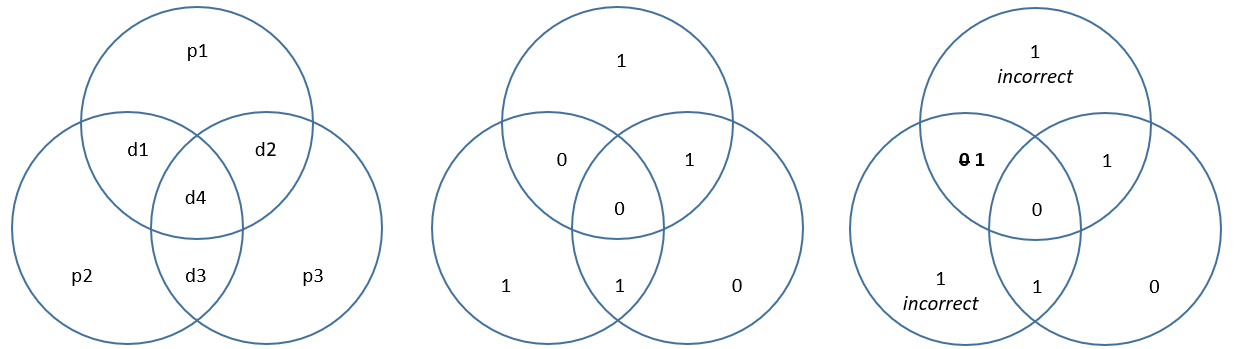
\includegraphics[width=\textwidth]{img/Hamming.png}
 \caption{Left: The basic structure of a Hamming (7, 4) code visualized as a sort of Venn diagram. The data bits, d1 through d4, form the intersections, and the parity bits, p1 through p4. Center: Data bits 0110 and the corresponding parity check bits. Right: A single bit error causes two parity checks to fail, allowing us to discern which bit was flipped.}
 \label{fig:hamming}
 \end{figure}

The data bits (labeled d1 through d4) form the overlapping regions of the Venn diagram. The parity bits are represented as the non-overlapping area. Within each circle of the diagram, the three data bits' sum should have the parity indicated by the parity bit. The example below shows how the three parity bits can be computed from the four data bits.

How does this help with error detection? Imagine if d1 is flipped from a 0 to a 1. Now, the parity of both p1 and p3 are incorrect, while the parity of p3 is correct. Knowing this, we know that d1 has been flipped, as in the center image.

What if a parity bit is flipped? Imagine if p1 has flipped from a 0 to a 1. In that case, we can tell that it's just the parity bit that flipped because the other two parity bits are correct.

The only other interesting case is if d4 flips, since d4 factors into all three parity bits. In that case, all three parity bits will be incorrect and we can pinpoint the error. \cite{wolf}

\subsection{Encoding and Decoding Hamming Codes}

A Hamming code begins by placing the parity bits at expected locations in the data, at the index powers of 2, so position 1, 2, 4, etc. This property actually shows that for larger Hamming codes, relatively fewer parity bits are required to correct a single error, since the powers of two will increasingly space out. To actually compute a Hamming Code in practice, we use matrix algebra. 

\begin{figure}[h!]
 \centering
 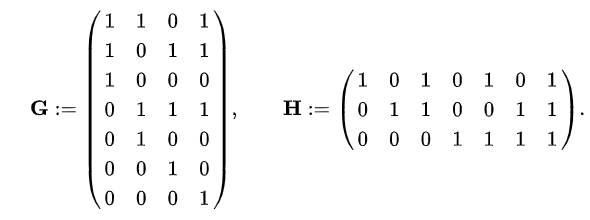
\includegraphics[width=.5\textwidth]{img/matrix.png}
 \caption{The two matrixes used for encoding and decoding Hamming codes in practice, a generator matrix $G$ and a parity check matrix $H$. \cite{wiki}}
 \label{fig:matrix}	
 \end{figure}

If we take $p$ as our initial data, and $x$ as the vector we intend to send, then we do the matrix multiplication $x = Gp$. G is a special matrix called a generator computed for the particular size of the Hamming Code which encapsulated the logic we discussed, computing and inserting the parity bits. This is always the same matrix for all data.

On receipt, we take the received codeword and multiply it by a different special matrix, called a parity check matrix, to get an output syndrome. Mathematically, this is $z = Hr$. $G$ and $H$ are shown in Figure \ref{fig:matrix}. The syndrome Z is will be a null vector if there are no errors, but if there is an error, its value modulo 2 will simply paint out the index of where the error is. We know which bits are the data bits, and so we can extract them, flip up to one error, and extract the transmitted codeword. \cite{wolf}

\subsection{Extended Hamming Codes}

A limitation of Hamming codes is that they only successfully correct a single bit error, and when multiple errors occur it can be detected because several parity bits will be off, but it is not possible to know exactly how many errors occurred. By adding an additional parity bit to the entire code, it becomes possible to determine if exactly two errors exist, using the same logic as correcting an error, but without the ability to determine exactly which two flipped. For network purposes, this is not particularly useful because any errors will trigger a retransmission, but for certain applications, knowing how many errors occurred can help with things like pinpointing hardware issues.

\section{Reed-Solomon Codes}

\subsection{Overview}

Hamming Codes are useful for correcting and detecting small numbers of errors. However, there are other classes of error that Hamming codes do not address. Burst errors, in particular, are common in physical media. Scratches on CDs can mess with a long run of data, and a burst of electrical noise can fry several bits in a row. Erasures can also occur if the media is able to communicate that an error has occurred but it is unsure what the correct value is, sort of like an "I don't know", perhaps if the medium detects noise or is able to determine that a value is not a strong 0 or a strong 1.

Reed-Solomon Codes are not a single code, but rather, a class of codes with different implementations that utilize a similar technique. In general, a Reed-Solomon code transforms a batch of bits into a block called a symbol. Each symbol is of a fixed size and therefore has a fixed total range of possible values. Reed-Solomon codes act by transforming the message symbols into values, coefficients, or other descriptor of a polynomial, or some mathematical product of a polynomial. The recipient takes advantage of mathematical properties of polynomials in order to determine which bits were incorrect. With Reed-Solomon, entire symbols are error-corrected. This means that a burst error that introduces noise to a large contiguous chunk of a message may only impact a small number of symbols, which can all then be corrected, making these very suitable for network and physical media applications. \cite{pless}

\subsection{How Reed-Solomon Codes work}

The critical property is that any distinct N points on a polynomial will uniquely determine the polynomial of degree at most N-1, that is, there is only one polynomial of degree N that has the specific N+1 points on it. As an example, how many horizontal lines (0 degree polynomials) go through a single point -- just one. How many lines (first degree polynomial) go through two points -- just one line. How many parabolas go through three points? Exactly one parabola. This continues for all degrees. We can exploit this property by, simplistically, describing a polynomial that fits the data symbols we are sending, and then add extra data points to the polynomial to over-define it, that is, use more symbols than we actually need to uniquely define it. Then, if there are errors, we can tease out which symbols don't match the same polynomial as the rest of the data points, and re-compute the correct point. \cite{tanenbaum}

As an example, take the polynomial below. The 8 points on it uniquely determine a polynomial of degree 7. That polynomial is drawn through the points and can be defined as an expression like $ax + bx^2 + cx^3 + dx^4 + ex^5 + fx^6 + gx^7$.

\begin{figure}[h!]
 \centering
 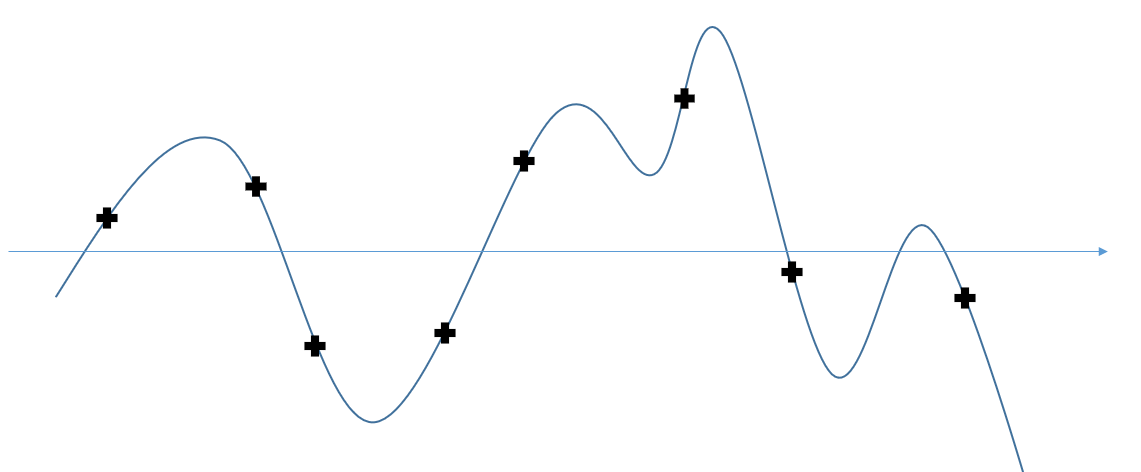
\includegraphics[width=0.5\textwidth]{img/poly1.png}
 \caption{Eight data symbols are plotted as data points on a polynomial of degree 7. That polynomial is uniquely defined.}
 \label{fig:poly1}
 \end{figure}

In an exaggerated drawing, we add redundant data points to the polynomial, and transmit that. This can be seen in Figure ~\ref{fig:poly2}.

\begin{figure}[h!]
 \centering
 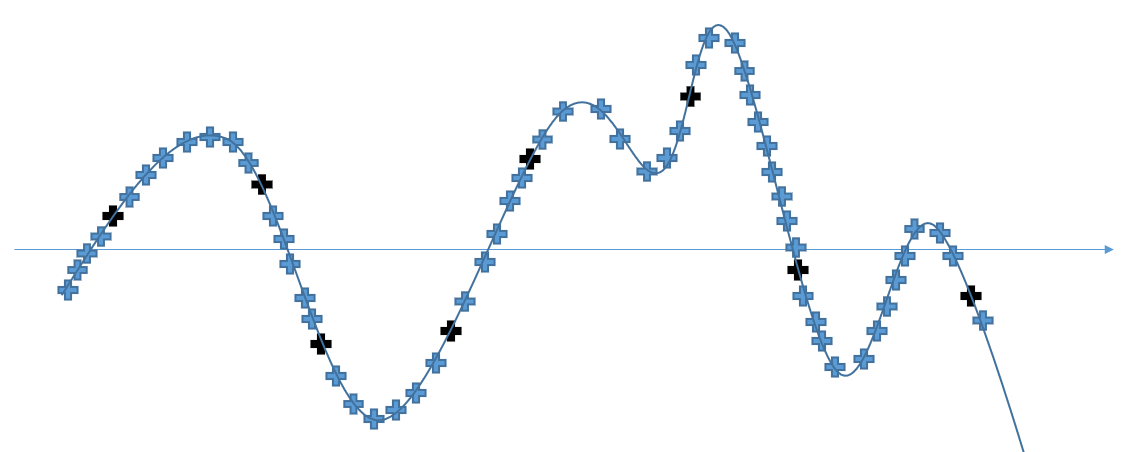
\includegraphics[width=0.5\textwidth]{img/poly2.png}
 \caption{We add more redundant data points at intervals along the same 7 degree polynomial (blue) along with the data (black) in order to over-define the polynomial.}
 \label{fig:poly2}
 \end{figure}

In transit, two errors occur. They are shown in green in ~\ref{fig:poly3}. Even in this simplified example, it becomes obvious that the redundant over-sampling of the polynomial means that the errors can be identified because they are the only data points that do not match the rest of the curve. Once they've been identified, we can re-compute the original polynomial using the redundant data points and determine the error-corrected placement of the symbols. 

\begin{figure}[h!]
 \centering
 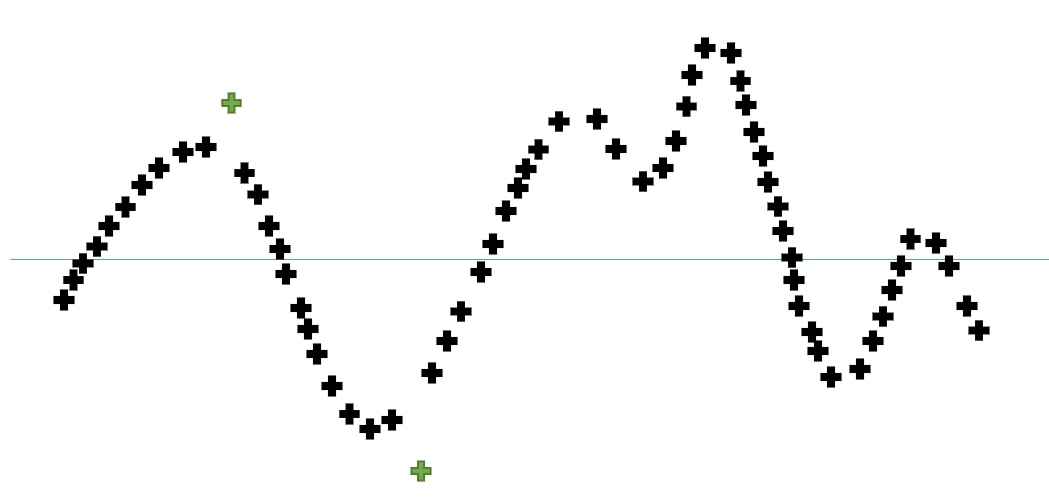
\includegraphics[width=0.5\textwidth]{img/poly3.png}
 \caption{Two errors occur in the transmitted data. Because the other data points match the same degree 7 polynomial, the two errors can be identified and corrected.}
 \label{fig:poly3}
 \end{figure}

 As you can see from this visual example, over-sampling the data enables us to recover the original polynomial, and once we have the original polynomial, it is trivial to re-compute any of the original symbols by simply evaluating the polynomial.

Reed-Solomon codes in practice utilize various techniques related to these. In the original view, Reed-Solomon codes utilized a strategy similar to what I described: the codewords are used as symbols in a polynomial, and all polynomials of degree K are computed for all possible groups of K+1 received symbols. Then, the most "popular" polynomial will be the correct one, since any polynomial that does not have an error will be the same, original one (Reed and Solomon 1960). However, this is tremendously inefficient since there are enormous numbers of combinations for large codes. Clearly we need a better approach.  \cite{rs}

\subsection{Encoding and Decoding Reed-Solomon Codes}

Reed-Solomon codes are, in practice, transmitted as codewords of N bytes, where there are K data bytes and N-K parity bytes. N-K is also referred to as 2t, as the value $t$ is used in computations. 

A heavily used code is RS(255,223) with symbols of 1 byte length. Codewords are 255 bytes, with 223 bytes as data and 32 bytes for parity. In that example, $n= 255, k = 223, s = 8, 2t = 32, t = 16$. A decoder can then correct up to 16 ($t$) symbol errors. 

In practice, Reed-Solomon codes are computed using what's known as a generator polynomial. A generator has the following form. Note that this has degree 2t. 

\begin{equation}
g(x) = (x-\alpha^i)(x-\alpha^(i+1))(x-\alpha^(i+2)) ... (x-\alpha^(i+2t))
\end{equation}

The codeword is computed as below: the symbols to transmit, i(x), are multipled by the generator at each index $x$. The codword, then, can be divided by the generator in order to determine the original information.

\begin{equation}
g(x) = g(x) * i(x)
\end{equation}

In addition, parity symbols are computed as well. These are computed by 

\begin{equation}
p(x) = i(x) * x^(n-k)  mod g(x)
\end{equation}

When the codeword is transmitted, there can be errors on the receiving side. The received codwords, r(x), is the transmitted codeword, c(x), plus any errors, e(x)/

\begin{equation}
r(x) = c(x) + e(x)
\end{equation}

On the receiving end, the receiver must follow a series of steps to determine if there are errors, where the errors are, and the corrected values. First, the error syndromes are computed, which is done by plugging the roots of the generator polynomial into $r(x)$. Once the syndromes are computed, the errror locations and values are computing using a pair of series of equations with $t$ unknowns. These can be done in practice fairly efficiently using Euclid's algorithm, the Berlekamp-Messey algorithm, and the Forney algorithm. These are computationally intensive, but high data rates can be achived on modern processors and efficient software code. \cite{rsg}

\section{Convolutional Codes}

A different approach to error correction are convolutional codes. Convolutional codes are not block codes because they do not operate on fixed blocks of data; rather, they operate on streams of data, continuously re-calculating the output bit value based on previous inputs. The output is deterministic and any errors will cause the output value to drift and no longer follow the expected summation logic. To correct errors, it is possible to figure out which bit error was the most likely culprit to cause the output sequence.

Convolutional codes are most useful for detecting single-bit errors on streams of data. They actually work well in tandem with block codes, because block codes like Reed-Solomon can very effectively correct bursts, and convolutional codes can correct single-bit errors. 

Convolutional codes are used in WiFi to improve reliability. WiFi is highly noisy and so overhead rates of 1/2 to 3/4 (to be discussed below) are used, depending on the data rate. It uses a 6-state shift register. % https://www.hamilton.ie/publications/xiaomin_thesis.pdf  

(Tanenbaum 231).

\subsection{Convolution Code Operation}

Convolutional codes utilize a sliding window to compute output parity bits based on the values of the input bits. As the window size increases, there is more capability for error correction, but it also becomes more difficult to compute errors; this is known as the constraint length. The number of parity bits, $r$, is independent of the constraint length; obviously more parity bits means more redundancy and a greater ability to correct errors. The data rate, then, is $\frac{1}{r}$, so it is best to optimize for modest constraint lengths to avoid computational complexity but also use a suitable small $r$ to reduce overhead. 

Interestingly, the output is entirely parity bits and so the actual data bits are never transmitted. 

A visualization is shown below. In the example here, $r$ is 3. The first parity bit sums all three bits, and the second sums the first and third bits.

\begin{figure}[h!]
 \centering
 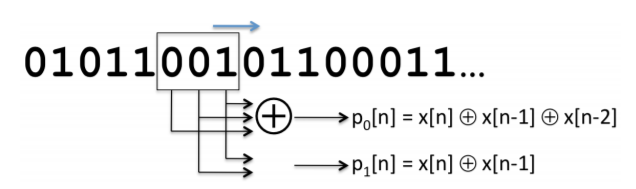
\includegraphics[width=0.5\textwidth]{img/conv.png}
 \caption{An example of a sliding window convolutional code operating on a stream of data. Three data bits are inspected to product two output parity bits. Source: } 
 \label{fig:conv}
 \end{figure}

These summations are known as parity equations and are a list of discrete equations. An example of possible parity equations with a sliding window length of 5 and three output parity bits are shown below for illustration.

\begin{equation}
  \begin{array}{l}
	p_0[n] = x[n] + x[n-1] + x[n-2] + x[n-3] + x[n-4] \\
	p_1[n] = x[n] + x[n-2] + x[n-4]  \\
	p_2[n] = x[n-2] + x[n-3] + x[n-4]
  \end{array} 
\end{equation}

These can also be written as the coefficients of each term in the sum, which can be thought of as a simple first degree polynomial. The above would be (1, 1, 1, 1, 1), (1, 0, 1, 0, 0), (0, 0, 1, 1, 1).

Each parity bit, then, has partial information about each actual data bit, depending on the coefficients chosen. So for this example, if we are trying to transmit a block of data that is 11111, the three parity bits would be 5 mod 2 = 1, 3 mod 2 = 1, 3 mod 2 = 1, or 111. \cite{rsg}

\subsection{Decoding}

Now that we have a suitable mechanism to add redundancy to our data, we need to be able to decode the original data from these. The approach used here is called a maximum likelihood decoder. A maximum likelihood decoder determines the input value that was most likely to produce the output value. With small constraint windows, such as n=4, we can simply try examine what all of the possible output bit streams could be, and then compute the Hamming distance between all of those and the received codeword. The lowest Hamming distance is the maximum likely transmitted data, because it requires the fewest changes.

Using our three-parity-bit equations from before, imagine we receive 110100000001 as our received codeword for a four-bit constraint window. This is not a valid code. If we manually compute all expected codewords and compute the Hamming distance from each codeword, we can see that the codeword for the input data 1010 only differs by a single bit, and therefore it is maximally likely that it is the case. \cite{rsg}

\begin{longtable}{| p{.20\textwidth} | p{.4\textwidth} | p{.2\textwidth} |} 
\hline
\textbf{Data} & \textbf{Code}    &     \textbf{Hamming Distance}  \\ \hline
0000 & 000000000000 & 4                \\ \hline
0001 & 000000000110 & 6                \\ \hline
0010 & 000000110100 & 7                \\ \hline
0011 & 000000110010 & 7                \\ \hline
0100 & 000110100111 & 6                \\ \hline
0101 & 000110100001 & 4                \\ \hline
0110 & 000110010011 & 5                \\ \hline
0111 & 000110010101 & 5                \\ \hline
1000 & 110100111101 & 4                \\ \hline
1001 & 110100111011 & 4                \\ \hline
1010 & 110100001001 & 1                \\ \hline
1011 & 110100001111 & 3                \\ \hline
1100 & 110010011010 & 6                \\ \hline
1101 & 110010011100 & 6                \\ \hline
1110 & 110010101110 & 7                \\ \hline
\caption{All possible output codewords for a given 4-bit convolutional decoder. The received codeword, 110100000001, only differs from the codeword for 1010 by 1 bit so we deduce that it is the most likely data.}
\label{tab:tab}
\end{longtable}

Because this type of code deals in probabilities of error, it is called a soft-decision encoding. Soft-decision encoding is useful for building a model of the likelihood of error. \cite{tanenbaum}

\subsection{Viterbi Decoding}

Another decoding approach is visualized using what's called a trellis. In Figure ~\ref{fig:trellis}, we see how the actual value output by a convolutional encoder traverses through the possible output values. The red path is that actual path taken.

\begin{figure}[ht!]
 \centering
 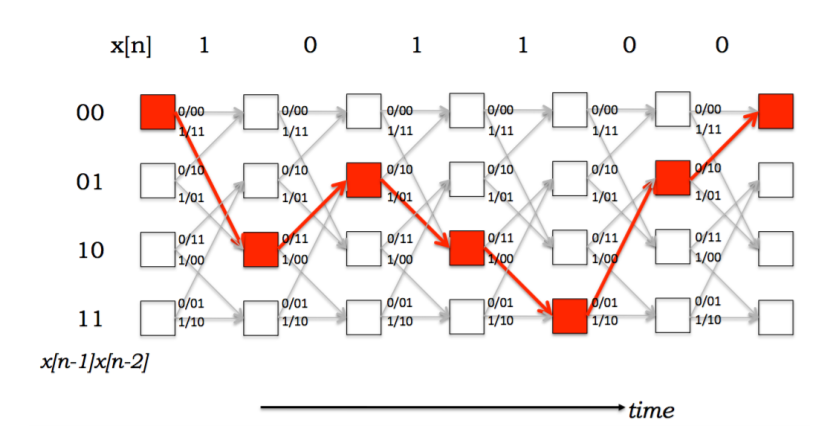
\includegraphics[width=0.75\textwidth]{img/trellis.png}
 \caption{An example of a sliding window convolutional code operating on a stream of data. Three data bits are inspected to product two output parity bits. \cite{mitconv} }
 \label{fig:trellis}
 \end{figure}

Each step through the trellis presents an opportunity to deviate from the received codeword due to an error. If a single error has occurred, then the path will have an error, but will eventually converge back to the correct path. The Viterbi decoder uses the Hamming distance as a way to measure the error at each step through the trellis for each given path state change. When an error has occured, there will be a non-zero Hamming distance at that point in the path compared to the received data. The Viterbi decoder, and the accompanying dynamic programming algorithm, minimize the total error by examining the state changes and produce the most likely original path. In doing so, it finds the most likely original data. This approach is more efficient than using the brute-force Hamming distance for all possible input data and can scale to larger constraint lengths. \cite{mitvit}

\section{Conclusion}

Error correction can be implemented using a variety of strategies, ranging from simple Hamming codes to complex Reed-Solomon codes. Error correcting codes help improve the WiFi user experience with convolution codes and help satellites transmit data effectively to Earth. They are a unique solution to a challenging problem inheret to communication channels.

\begin{thebibliography}{9}

\bibitem{tanenbaum} 
Tanenbaum, Andrew S., and D Wetherall. Computer networks. Boston: Pearson Prentice Hall, 2011. Print.
 
\bibitem{mitconv} 
MIT 6.02 DRAFT Lecture Notes, Lecture 8: Convolutional Coding. Fall 2010. 
\\\texttt{http://web.mit.edu/6.02/www/f2010/handouts/lectures/L8.pdf}

\bibitem{mitvit} 
MIT 6.02 DRAFT Lecture Notes, Lecture 9: Viterbi Decoding of Convolutional Codes. Fall 2010.
\\\texttt{http://web.mit.edu/6.02/www/f2010/handouts/lectures/L9.pdf}

\bibitem{rsg} 
Riley, Martyn and Richardson, Iain. An introduction to Reed-Solomon codes: principles, architecture and implementation. Carnegie Mellon University.
\\\texttt{https://www.cs.cmu.edu/\textasciitilde{}guyb/realworld/reedsolomon/reed\_solomon\_codes.html}

\bibitem{pless}
Pless, Vera. Introduction to the theory of error-correcting codes. New York: Wiley, 1998. Print.

\bibitem{wolf}
Wolf, Jack Keil. AN INTRODUCTION TO ERROR CORRECTING CODES: Part 1. University of California, San Diego. Spring 2018. \texttt{http://circuit.ucsd.edu/\textasciitilde{}yhk/ece154c-spr17/pdfs/ErrorCorrectionI.pdf}

\bibitem{duke}
Reed-Solomon Codes. Duke University Computer Science. \texttt{https://www2.cs.duke.edu/courses/spring10/cps296.3/rs\_scribe.pdf
}

\bibitem{sphere}
Leech, John and Sloane, N. J. A. SPHERE PACKINGS AND ERROR-CORRECTING CODES. Can. J. Math., Vol. XXIII, No. 4, 1971, pp. 718-745. \texttt{https://pdfs.semanticscholar.org/1ad2/f4381226d6e5ef815f3ea1fba3616e5c5d10.pdf}

\bibitem{wiki}
Hamming(7,4). Wikipedia: The Free Encyclopedia. \texttt{https://en.wikipedia.org/wiki/Hamming(7,4)}

\bibitem{rswiki}
Reed-Solomon Error Correction. Wikipedia: The Free Encyclopedia. \texttt{https://en.wikipedia.org/wiki/Reed\%E2\%80\%93Solomon\_error\_correction
}

\bibitem{rs}
Solomon, G. and Reed, I.S. Polynomial Codes Over Certain Finite Fields. Journal of the Society for Industrial and Applied Mathematics, 8(2), 300–304. \texttt{https://epubs.siam.org/doi/10.1137/0108018}

\end{thebibliography}

\end{document}
